\section{ХОД РАБОТЫ}

\subsection{Формулировка задачи}

Требуется вывести на экран монитора графики поверхностей и линии равных
уровней плотностей вероятности приведенных выше двухмерных распределений
(при $ k = 2 $ ) и исследовать их зависимость от параметров распределений.

Для нормального распределения в одно графическое окно вывести эллипс
рассеяния и две функции регрессии. Исследовать зависимость формы и
площади эллипса рассеяния от коэффициента корреляции при заданных дисперсиях
компонент случайного вектора. Исследовать взаимное расположение
функций регрессии и осей эллипса рассеяния (совпадают ли функции регрессии
с осями эллипса?).

\subsection{Теоретические сведения}

Плотность вероятности \textit{двухмерного нормального распределения}:
\begin{equation}
    f_{\overline{\xi}}(x_1, x_2) =
    \dfrac{1}{2 \pi \sigma_1 \sigma_2 \sqrt{1-r_{1,2}^2}} \hspace{1mm} exp \Big(-\dfrac{1}{2}\phi(x_1, x_2) \Big),
\end{equation}

\noindent где параметр $ \phi(x_1, x_2) $ определяется следующим образом: 

\begin{equation*}
    \phi(x_1, x_2) = \dfrac{1}{1-r_{1,2}^2}
    \Bigg(
    \dfrac{(x_1 - a_1)^2}{\sigma_1^2} - 
    2r_{1,2} \dfrac{(x_1 - a_1)}{\sigma_1} \dfrac{(x_2 - a_2)}{\sigma_2} +
    \dfrac{(x_2 - a_2)^2}{\sigma_2^2} 
    \Bigg).
\end{equation*}

Плотность вероятности \textit{произведения одномерных гамма-распределений}:
\begin{equation}
    \begin{aligned}
      f_{\overline{\xi}}(\overline{x}) =
      \left\{
        \begin{aligned}
          &\prod_{i=1}^m \dfrac{1}{\Gamma(a_i)b_i^{a_i}} x_i^{a_i-1} e^{-\dfrac{x_i}{b_i}}, \hspace{3mm} &x_i > 0, b_i > 0, a_i > 0, \\
          &0, \hspace{11.5mm} &x \le a.
        \end{aligned}
      \right.
    \end{aligned}
  \end{equation}

\subsection{Многомерное нормальное распределение}

Графики поверхностей двухмерного нормального распределения представлены
на рисунках~\ref{pic:normal_mesh_start}--\ref{pic:normal_mesh_end}.

\begin{figure}[h!]
  \begin{minipage}[h!]{0.47\linewidth}
    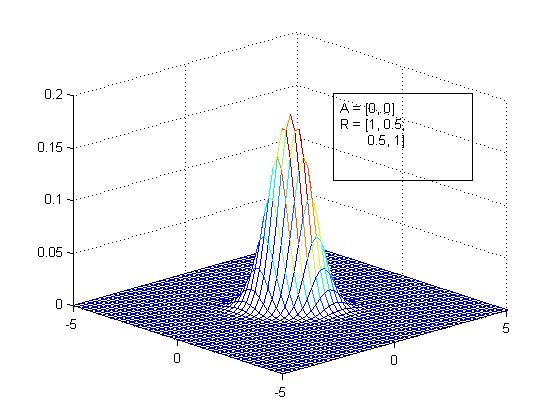
\includegraphics[width=1\linewidth]{pic/new/normal_mesh_1}
    \caption{П.~в. нормального распределения при
    $ R = \big[1, 0.5, 0.5, 1 \big] $
  }
    \label{pic:normal_mesh_start}
  \end{minipage}
  \hfill
  \begin{minipage}[h!]{0.47\linewidth}
    \vspace{4mm}
    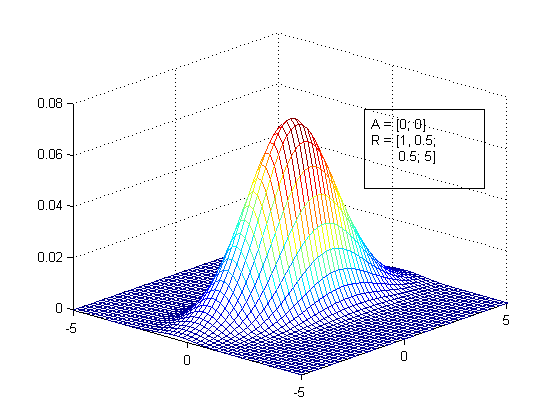
\includegraphics[width=1\linewidth]{pic/new/normal_mesh_2}
    \caption{П.~в. нормального распределения при
    $ R = \big[1, 0.5, 0.5, 5 \big] $}
  \end{minipage}
\end{figure}

\begin{figure}[h!]
  \begin{minipage}[h!]{0.47\linewidth}
    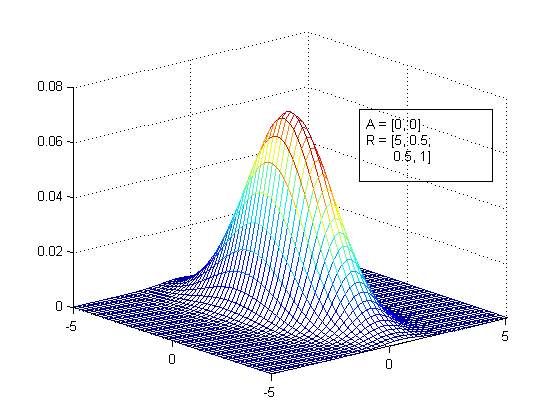
\includegraphics[width=1\linewidth]{pic/new/normal_mesh_3}
    \caption{П.~в. нормального распределения при
    $ R = \big[5, 0.5, 0.5, 1 \big] $}
  \end{minipage}
  \hfill
  \begin{minipage}[h!]{0.47\linewidth}
    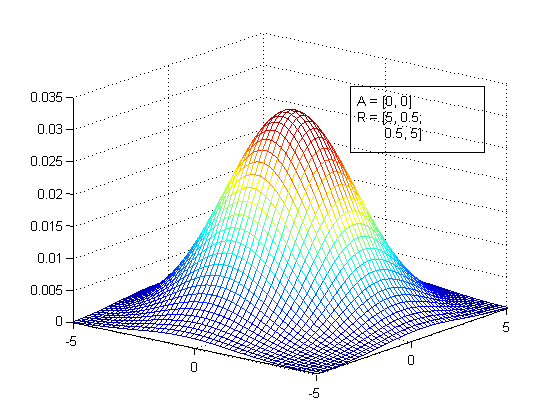
\includegraphics[width=1\linewidth]{pic/new/normal_mesh_4}
    \caption{П.~в. нормального распределения при
    $ R = \big[5, 0.5, 0.5, 5 \big] $}
    \label{pic:normal_mesh_end}
  \end{minipage}
\end{figure}

\newpage

Графики линий равных уровней плотности вероятности нормального распределения при различных
параметрах приведены на рисунках~\ref{pic:normal_contour_start}--\ref{pic:normal_contour_end}.

\begin{figure}[h!]
  \begin{minipage}[h!]{0.47\linewidth}
    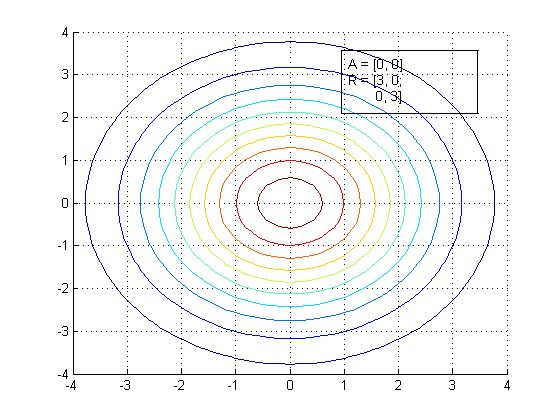
\includegraphics[width=1\linewidth]{pic/new/normal_contour_1}
    \caption{линии уровня п.~в.
      нормального распределения при $ R = \big[3, 0, 0, 3 \big] $}
    \label{pic:normal_contour_start}
  \end{minipage}
  \hfill
  \begin{minipage}[h!]{0.47\linewidth}
    \vspace{4mm}
    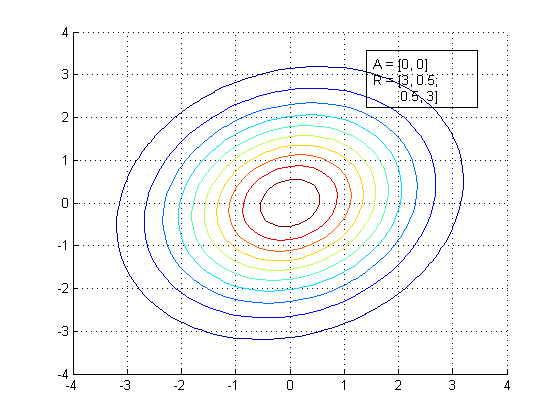
\includegraphics[width=1\linewidth]{pic/new/normal_contour_2}
    \caption{линии уровня п.~в.
      нормального распределения при $ R = \big[3, 0.5, 0.5, 3 \big] $}
  \end{minipage}
\end{figure}

\begin{figure}[h!]
  \centering
  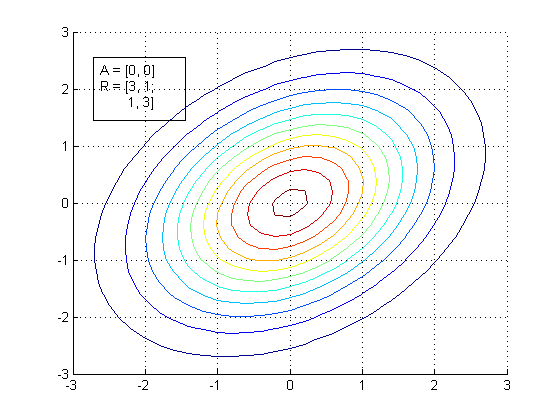
\includegraphics[width=0.5\linewidth]{pic/new/normal_contour_3}
  \caption{линии уровня п.~в. \\
    нормального распределения при \\
    $ R = \big[3, 1, 1, 3 \big] $}
  \label{pic:normal_contour_end}
\end{figure}

\newpage 

\subsection{Произведение одномерных гамма-распределений}

Графики поверхностей произведения одномерных гамма-распределений
продемонстрированы 
на рисунках~\ref{pic:gamma_mesh_start}--\ref{pic:gamma_mesh_end}.

\begin{figure}[h!]
  \begin{minipage}[h!]{0.47\linewidth}
    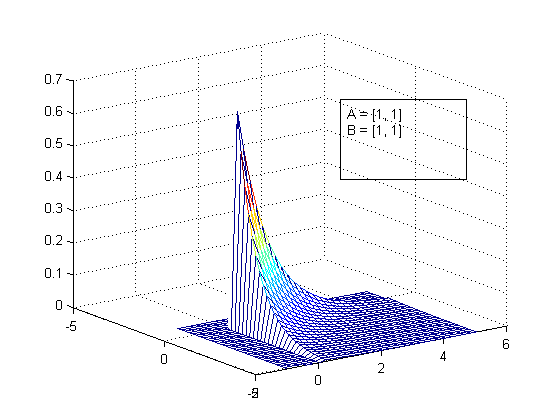
\includegraphics[width=1\linewidth]{pic/new/gamma_mesh_1}
    \caption{П.~в. произведения одномерных гамма-распределений при 
    $ A = \big[1, 1\big], B = \big[ 1, 1 \big] $
    }\label{pic:gamma_mesh_start}
  \end{minipage}
  \hfill
  \begin{minipage}[h!]{0.47\linewidth}
    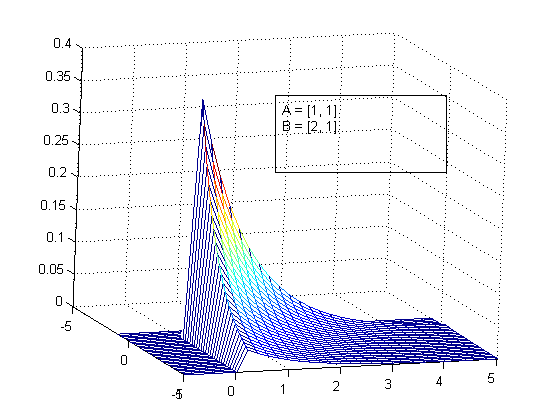
\includegraphics[width=1\linewidth]{pic/new/gamma_mesh_2}
    \caption{П.~в. произведения одномерных гамма-распределений при 
      $ A = \big[1, 1\big], B = \big[ 2, 1 \big] $}
  \end{minipage}
\end{figure}

\begin{figure}[h!]
  \begin{minipage}[h!]{0.47\linewidth}
    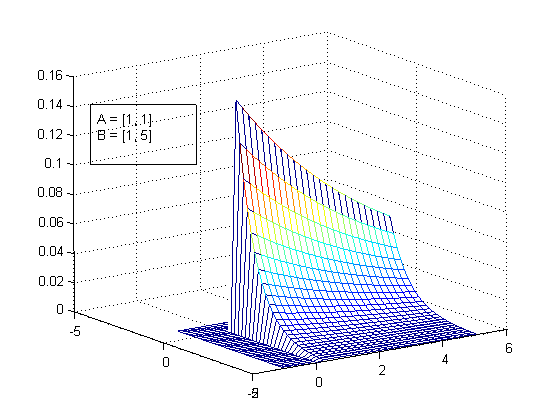
\includegraphics[width=1\linewidth]{pic/new/gamma_mesh_3}
    \caption{П.~в. произведения одномерных гамма-распределений при
      $ A = \big[1, 1\big], B = \big[ 1, 5 \big] $}
  \end{minipage}
  \hfill
  \begin{minipage}[h!]{0.47\linewidth}
    \vspace{4mm}
    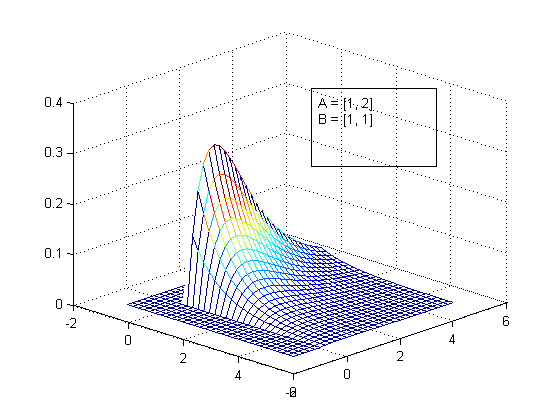
\includegraphics[width=1\linewidth]{pic/new/gamma_mesh_4}
    \caption{П.~в. произведения одномерных гамма-распределений при
      $ A = \big[1, 2\big], B = \big[ 1, 1 \big] $}
  \end{minipage}
\end{figure}

\newpage

\begin{figure}[h!]
  \begin{minipage}[h!]{0.47\linewidth}
    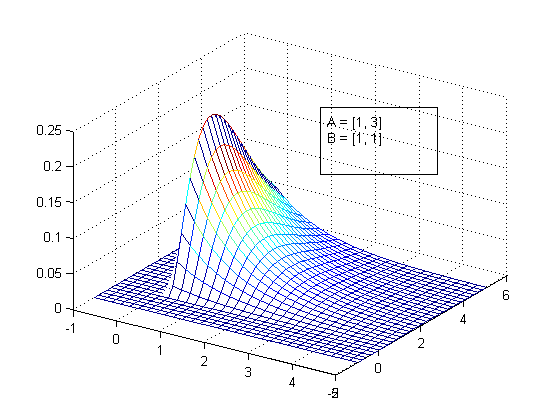
\includegraphics[width=1\linewidth]{pic/new/gamma_mesh_5}
    \caption{П.~в. произведения одномерных гамма-распределений при 
      $ A = \big[1, 3\big], B = \big[ 1, 1 \big] $}
  \end{minipage}
  \hfill
  \begin{minipage}[h!]{0.47\linewidth}
    \vspace{4mm}
    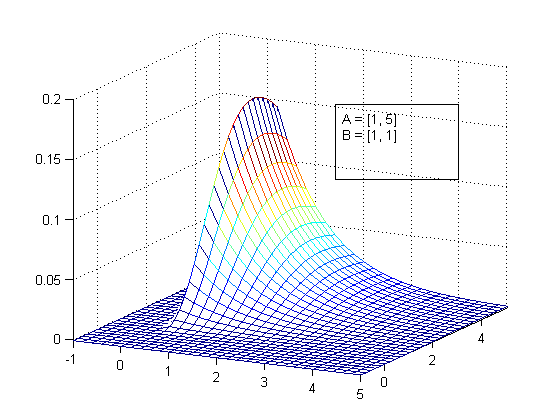
\includegraphics[width=1\linewidth]{pic/new/gamma_mesh_6}
    \caption{П.~в. произведения одномерных гамма-распределений при
      $ A = \big[1, 5\big], B = \big[ 1, 1 \big] $}
  \end{minipage}
\end{figure}

\begin{figure}[h!]
  \centering
  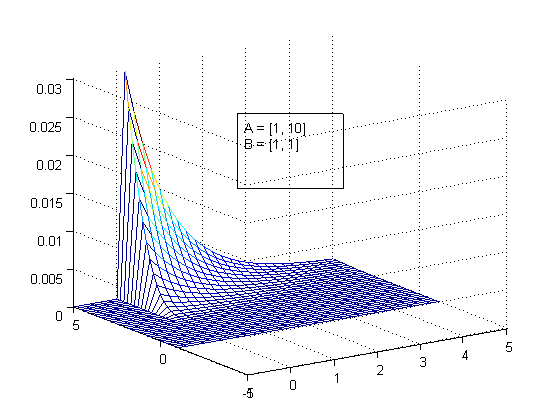
\includegraphics[width=0.5\linewidth]{pic/new/gamma_mesh_7}
  \caption{П.~в. произведения \\ одномерных гамма-распределений \\
    при $ A = \big[1, 10\big], B = \big[ 1, 1 \big] $}\label{pic:gamma_mesh_end}
\end{figure}

\newpage

Графики линий равных уровней плотности вероятности гамма-распределений при различных
параметрах приведены на рисунках~\ref{pic:gamma_contour_start}~-~\ref{pic:gamma_contour_end}.

\begin{figure}[h!]
  \begin{minipage}[h!]{0.47\linewidth}
    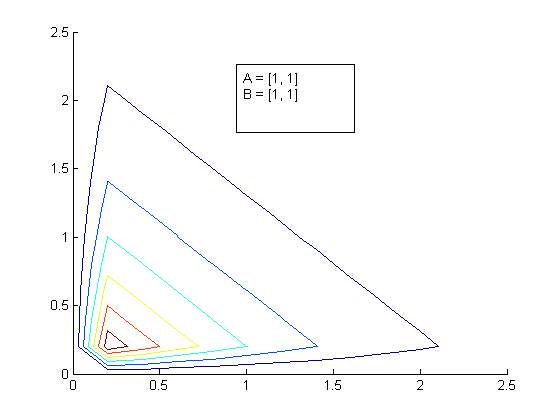
\includegraphics[width=1\linewidth]{pic/gamma_contour_1}
    \caption{Линии уровня п.~в. произведения одномерных гамма-распределений при
      $ A = \big[1, 1\big], B = \big[ 1, 1 \big] $}
    \label{pic:gamma_contour_start}
  \end{minipage}
  \hfill
  \begin{minipage}[h!]{0.47\linewidth}
    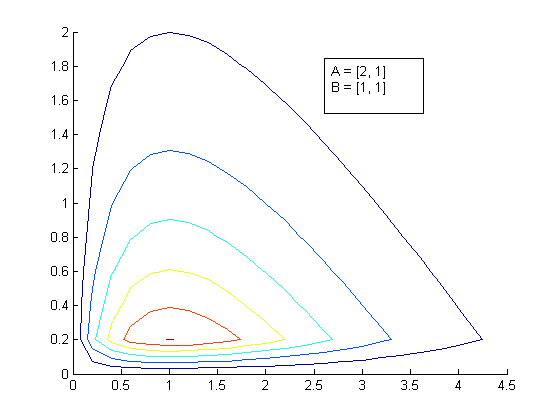
\includegraphics[width=1\linewidth]{pic/gamma_contour_2}
    \caption{Линии уровня п.~в. произведения одномерных гамма-распределений при
      $ A = \big[2, 1\big], B = \big[ 1, 1 \big] $}
  \end{minipage}
\end{figure}

\begin{figure}[h!]
  \centering
  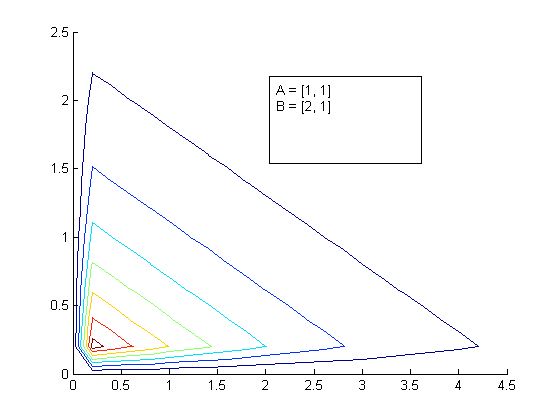
\includegraphics[width=0.5\linewidth]{pic/gamma_contour_3}
  \caption{Линии уровня п.~в произведения одномерных 
    гамма-распределений при
      $ A = \big[2, 1\big], B = \big[ 2, 1 \big] $}
  \label{pic:gamma_contour_end}
\end{figure}

\newpage

\subsection{Функции регрессии двухмерного
  нормального распределения}

Зависимость эллипса рассеяния и функций регрессии от параметров распределения изображена на рисунках~\ref{pic:normal_regr_start}--\ref{pic:normal_regr_end}.

\begin{figure}[h!]
  \begin{minipage}[h!]{0.47\linewidth}
    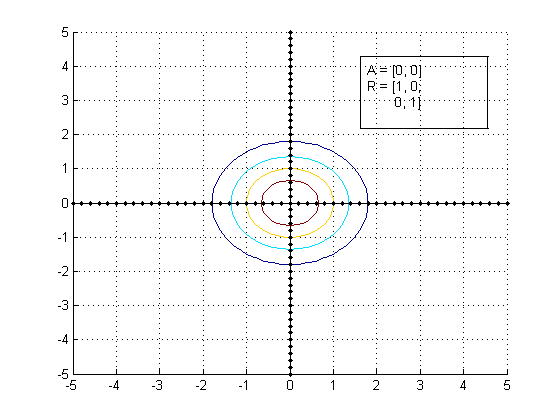
\includegraphics[width=1\linewidth]{pic/new/normal_regr_1}
    \caption{Эллипс рассеяния и функции регрессии 
       нормального распределения при
    $ R = \big[1, 0, 0, 1 \big] $
}\label{pic:normal_regr_start}
  \end{minipage}
  \hfill
  \begin{minipage}[h!]{0.47\linewidth}
    \vspace{4mm}
    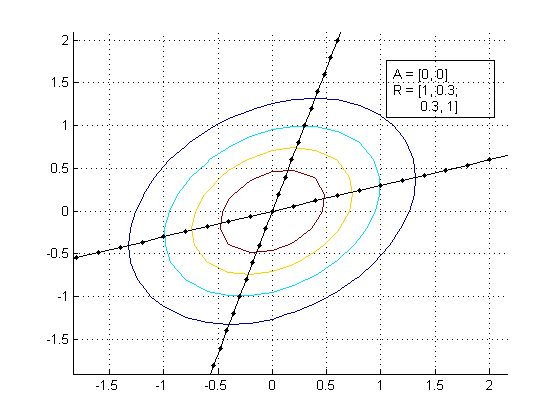
\includegraphics[width=1\linewidth]{pic/new/normal_regr_2}
    \caption{Эллипс рассеяния и функции регрессии 
       нормального распределения при
      $ R = \big[1, 0.3, 0.3, 1 \big] $
    }
  \end{minipage}
\end{figure}

\begin{figure}[h!]
  \begin{minipage}[h!]{0.47\linewidth}
    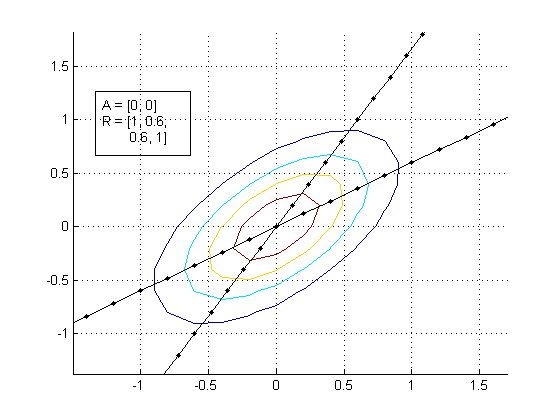
\includegraphics[width=1\linewidth]{pic/new/normal_regr_3}
    \caption{График эллипса рассеяния и двух функций регрессии при
      $ R = \big[1, 0.6, 0.6, 1 \big] $}
  \end{minipage}
  \hfill
  \begin{minipage}[h!]{0.47\linewidth}
    \vspace{4mm}
    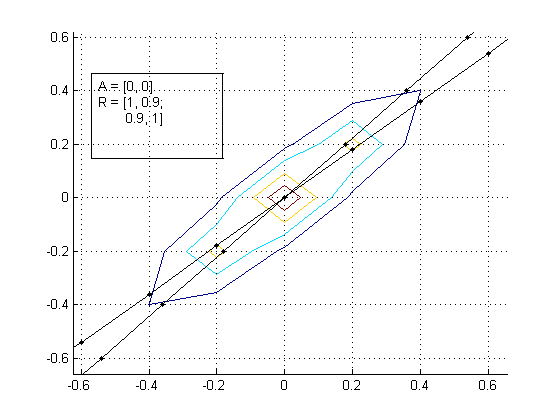
\includegraphics[width=1\linewidth]{pic/new/normal_regr_4}
    \caption{Эллипс рассеяния и функции регрессии 
       нормального распределения при
      $ R = \big[1, 0.9, 0.9, 1 \big] $
    }\label{pic:normal_regr_end}
  \end{minipage}
\end{figure}

\newpage
